\documentclass{article}
\usepackage{subcaption}
\usepackage{graphicx}
\usepackage{mathtools}
\usepackage{amssymb}
\usepackage{setspace}
\usepackage{hyperref}
\usepackage{float}

% code to adjust margins
\addtolength{\oddsidemargin}{-.875in}
	\addtolength{\evensidemargin}{-.875in}
	\addtolength{\textwidth}{1.75in}

	\addtolength{\topmargin}{-.875in}
	\addtolength{\textheight}{1.75in}

\makeatletter

\title{Probability Project Observations}
\author{Omema Ahmed oa04320 \\ Aiman Junaid aj05161 \\ Fatima Zehra fz04316}
\date{\today}
\begin{document}
    \maketitle
    \begin{center}
        \href{https://github.com/habib-university/Probability-Project---Random-Walk}{GitHub Repository Link - Random Walk Codes}
    \end{center}
    \section*{Task 1}
    To find the expected distance from the starting point (i.e. origin by default or the given coordinates), we ran simulations for 10000 walks and calculated their average.
    Our function increments the distance of a random walk at each step, which is 1 in our case, and returns its sum. Negative coordinates denote movement on left of origin, 
    and positive denote movement on right. To move left, we subtract 1 from x, and to move right we add 1.
    The shape of our resulting graph was a Gaussian curve, which is because binomial converges to Normal distribution. % insert reference to figure
    We tested our model for a range of probabilities, and each gives a different expected distance based on their probabilities and starting position.

    \section*{Task 2}
    To calculate the expected time for two random walks to meet, we calculated the total steps it took both of them to reach the same x-coordinate, and ran simulation for 10000 walks to take average.
    In our function, we started one walk from x=0, and randomly assigned the starting position of second walk. We tested our model for unequal probabilities, for one position being fixed (not moving), 
    and for different starting position of both walks.
    The resulting graph displays that the time it took for most of them to meet, was within 5000 steps.
    
    \section*{Task 3}
    To simulate a 2D random walk, we used matplotlib's animation. Our model is based on the theory of brownian motion. If the particle moves past 
    the boundary of the circle i.e. the circumference of the circle, the particle reflects on the surface on the circle and bounces back 
    inside the circle. If the angle of incidence on the surface of the circle is $\theta$, then the angle of reflection will also be $/theta$, and the angle with x-axis with which it will bounce
    back inside the circle would be $\frac{3\pi}{2} - \theta$, using bearing of circle. One assumption that we made is that, if the angle with which it will bounce back comes as one that reflects the particle 
    outside the bounds of the circle, then we keep calculating new angle until it reflects inside the circle.
    The distance with which the particle will bounce is equal to the difference between the line from origin and current point and the line from origin to the point outside the circle (new point).
    
    \section*{Task 4}
    We used a uniform random variable, and calculated the step size that ranged between 0-1, using numpy's random.uniform() function.
    Our resulting graph was a Gaussian curve, but in comparison with \textbf{Task 1}, it is smoother as we used continuous values for step.
    Again, we calculated the expected distance using the same method as explained earlier for \textbf{Task 1}.

    \section*{Task 5}
    To simulate the 2D random walk using uniform random variables for both the orientation and steps, we used numpy's random.uniform() function, and it gives us floating point numbers in the given range.
    The graph that it generates is more concentrated at the origin i.e it is densely populated instead of the one like in \textbf{Task 3}, using discrete values where it sparsed.

    \section*{Task 7}
    In this 2D random walk model, using discrete and continuous random variable for step size and orientation respectively, we get a graph which is populated at the origin due to continuous random variable for 
    orientation.

    \section*{Task 8}
    For this task, we simulated two random walks together, starting at different random locations within the boundary of the circle. The position we chose for each was randomly calculated by the formula $rcos(\theta)$ for x-coordinate
     and $rsin(\theta)$ for y-coordinate. After each step in the random walk, we calculated by distance between the two particles and when it became $< 1$, we stop the walks. We ran the simulation 10000 times, summed up the total number for steps for all simulations,
     and calculated average by dividing it by 10000, to get the expected number of steps for two random walks to collide.
    \section*{Graphs}
    % How to insert images
    \begin{figure}[H]
        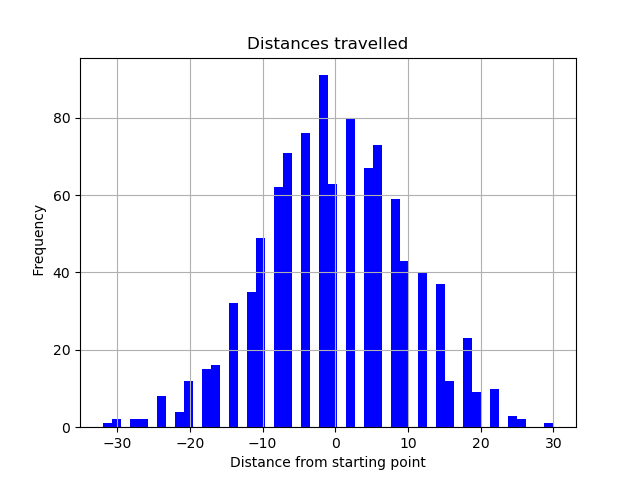
\includegraphics[width=15cm]{Graphs/task1.png}
        \centering
        \caption{\textbf{Task 1 (Discrete Random Variables)}}
    \end{figure}
    \begin{figure}[H]
        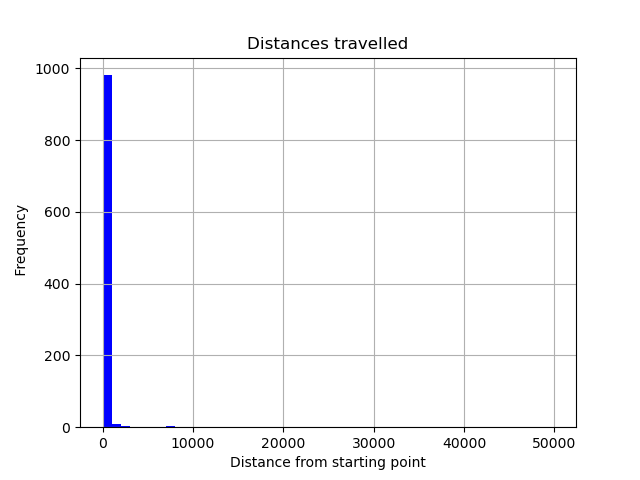
\includegraphics[width=15cm]{Graphs/task2.png}
        \centering
        \caption{\textbf{Task 2 (Discrete Random Variables)}}
    \end{figure}
    \begin{figure}[H]
        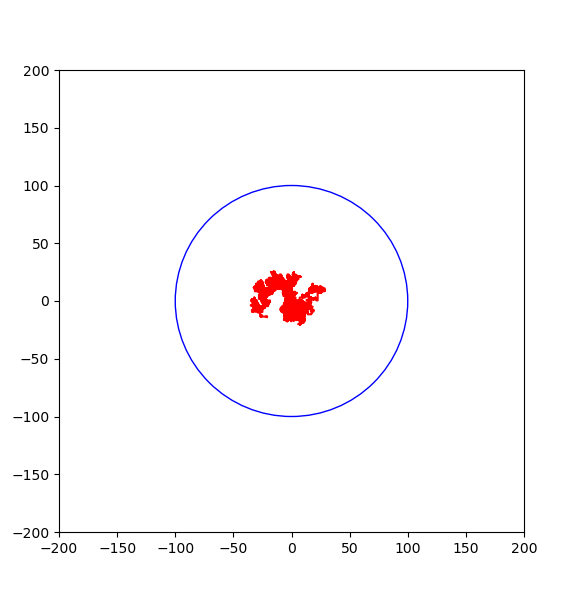
\includegraphics[width=15cm]{Graphs/task3.png}
        \centering
        \caption{\textbf{Task 3 (Discrete Random Variables)}}
    \end{figure}
    \begin{figure}[H]
        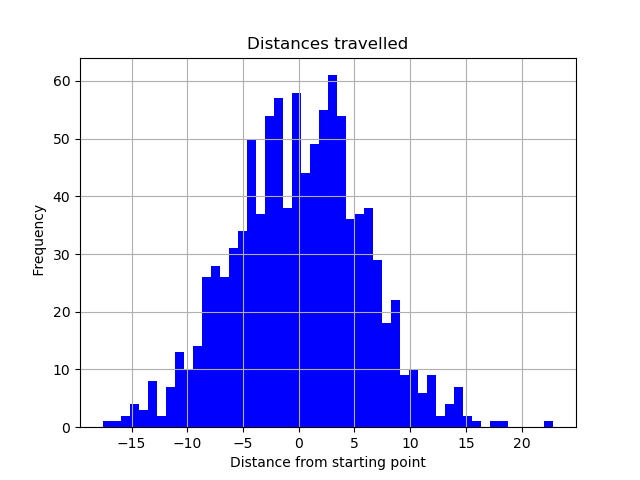
\includegraphics[width=15cm]{Graphs/task4.png}
        \centering
        \caption{\textbf{Task 4 (Continuous Random Variables)}}
    \end{figure}
    \begin{figure}[H]
        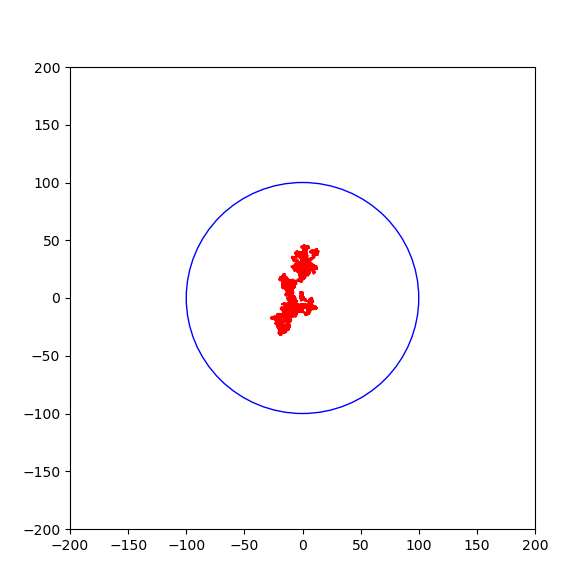
\includegraphics[width=15cm]{Graphs/task5.png}
        \centering
        \caption{\textbf{Task 5 (Discrete Random Variables)}}
    \end{figure}
    \begin{figure}[H]
        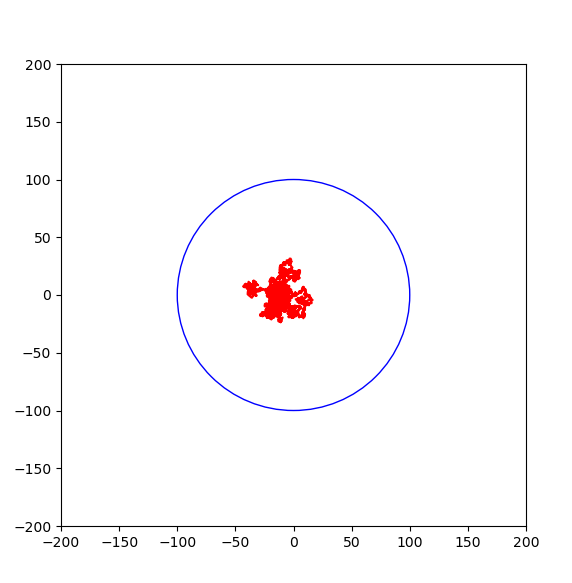
\includegraphics[width=15cm]{Graphs/task7.png}
        \centering
        \caption{Task 7 (Discrete Random Variables)}
    \end{figure}
    \begin{figure}[H]
        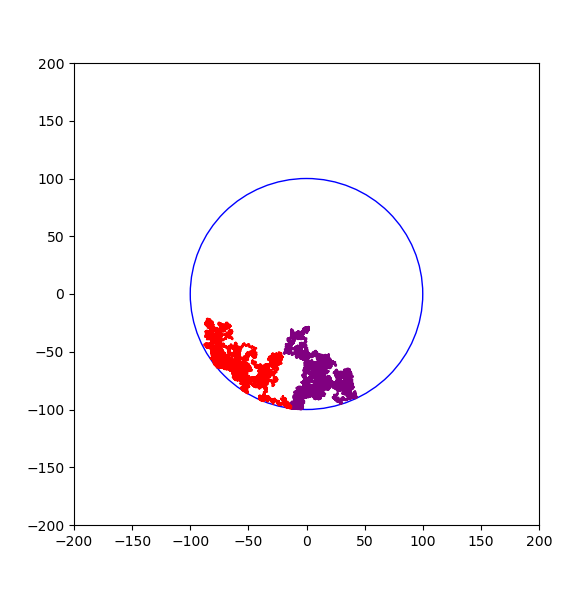
\includegraphics[width=15cm]{Graphs/task8.png}
        \centering
        \caption{\textbf{Task 8}}
    \end{figure}
    
    \section*{Bibliography}
    \begin{itemize}
        \item \href{http://web.mit.edu8.334/www/grades/projects/projects17/OscarMickelin/brownian.html}{Random Walk \& Brownian Motion}
        \item \href{https://www.math.uchicago.edu/~lawler/reu.pdf}{Random Walk \& Heat Equation}
        \item \href{https://books.google.com.pk/books?id=U2CrDY1MH5kC&pg=PA374&lpg=PA374&dq=how+to+reflect+a+point+from+the+boundary+of+circle+in+random+walk&source=bl&ots=_rt0N7oorr&sig=ACfU3U1LqlLgMpwvczXGymF0JxRteDJoRw&hl=en&sa=X&ved=2ahUKEwjP0PnOn47qAhUMqxoKHRbkCfwQ6AEwC3oECAkQAQ#v=onepage&q=how%20to%20reflect%20a%20point%20from%20the%20boundary%20of%20circle%20in%20random%20walk&f=false}{Mathematical Computing: An Introduction to Programming Using Maple}
        \item \href{http://physics.gu.se/~frtbm/joomla/media/mydocs/LennartSjogren/kap2.pdf}{Random Walks}
        \item \href{https://matplotlib.org/tutorials/introductory/pyplot.html}{Matplotlib Syntax}
    \end{itemize}
\end{document}